\documentclass[letterpaper, 11pt]{article}
\usepackage{comment} % enables the use of multi-line comments (\ifx \fi) 
\usepackage{fullpage} % changes the margin
\usepackage{fancyhdr} % for footer
\usepackage[UKenglish]{isodate}% http://ctan.org/pkg/isodate for date format
\usepackage[]{natbib}
\usepackage{hyperref}
\usepackage{graphicx}
\usepackage{wrapfig}
\usepackage[normalem]{ulem}%for strikethrough
\usepackage[font={small,sf}]{caption}
\usepackage{epigrafica}%changes default font to epigrafica
\usepackage{csquotes}%for blockquote

\pagestyle{fancy}
\renewcommand{\headrulewidth}{0pt}

\lhead{}
\chead{}
\rhead{}
\lfoot{ENT 432 (Fall 2017) - Penn State}
\cfoot{}
\rfoot{\thepage}
\renewcommand{\footrulewidth}{0.4pt}
\title{Discover your inner Darwin: insect observation and collection}
\author{Open Entomology Project}
\def\labelitemi{--}

\begin{document}
\cleanlookdateon %removed ordinal date
\maketitle
\thispagestyle{fancy}

\section*{Background}
\begin{wrapfigure}{r}{0.4\textwidth}
  \vspace{-24pt}
  \begin{center}
    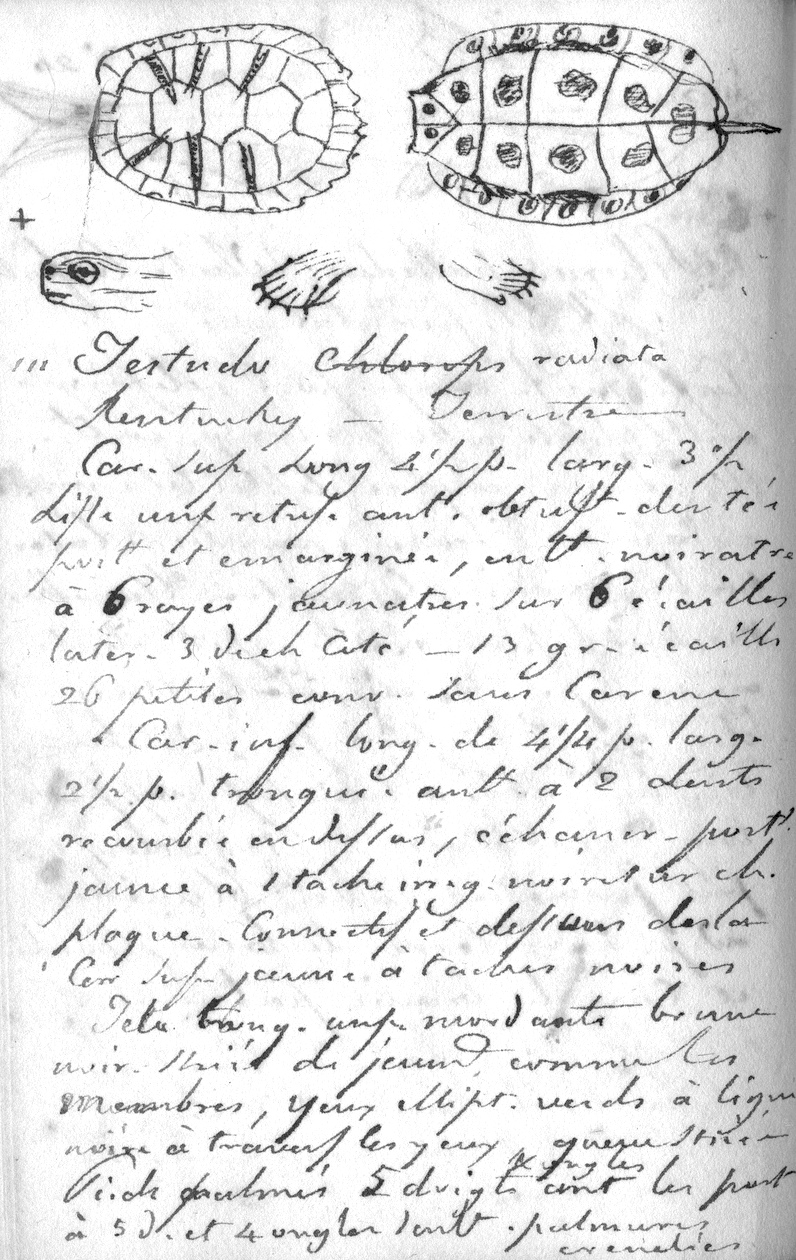
\includegraphics[width=0.36\textwidth]{Rafinesque}%Dyer https://flic.kr/p/FUBois
  \end{center}
  \vspace{-17pt}
  \caption{A page from Constantine Rafinesque's (1818) field notebook. What would a page from yours look like? See original image: \url{https://flic.kr/p/dbEePV}}
  \vspace{-30pt}
\end{wrapfigure}

Entomology is informed, enriched, and inspired by a broad knowledge of natural history, what \cite{Tewksbury01042014} refer to as the ``fundamental properties of organisms''. We cover natural history extensively in lecture discussions and lab exercises---what insects eat, how they reproduce, how to diagnose taxa, how different groups are related, adaptations they have, how they interact with symbionts, parasites, predators, \textit{etc}. To really understand and appreciate insects, though, there is no substitute for time spent carefully observing these organisms in their natural environment and in the lab, under the microscope. \\

\noindent{}For this exercise you will do just that---carefully observe and document insect life. You will keep extensive field notes about what you see, and you will collect specimens that serve as vouchers for your observations. This insect collection will be extended through subsequent collecting, the details of which are described below.

\section*{Graded products}

\subsection*{1. Field journal (100 pts.)}
The journal serves as the record of your natural history observations and their environmental context (``these things'' in the quote below). It will contain data about insects, but it may also include sketches, thoughts, stories, hypotheses, haiku, notes about what to do in future observations, \textit{etc}. We will provide you with a field journal that is archival and water resistant (Rite In The Rain No: 371FX, 4 5/8 $\times$ 7$''$, 48 pages). \textit{This notebook is property of the Frost Entomological Museum and must be deposited there at the end of the semester.} You should use only pencil or an \textit{archival} ink pen (\textit{e.g.}, Sakura\textregistered{ }Pigma Micron\textregistered; \url{http://www.pigmamicron.com/museums}); neither of these is provided. The field journal should be turned in with your collection on the last day of class, and all of your specimens should be documented in it.

\paragraph{Notes on strategy:} The field journal is a substantial portion of your grade, and people will have free access to the final product, in perpetuity. This quote from \citet[][pages 44--45]{bhl86279}, as highlighted by \cite{herman1986naturalist}, eloquently describes the approach you should take in journaling:\vspace{1mm}
\begin{displayquote}\small
Now \textit{you} know these things, but very likely no one else does ; and you know them \textit{at the time}, but you will not recollect a tithe of them in a few weeks or months, to say nothing of years. Don't trust your memory ; it will trip you up ; what is clear now will grow obscure ; what is found will be lost. Write down everything while it is fresh in your mind ; write it out in full --- time so spent now will be time saved in the end, when you offer your researches to the discriminating public. Don't be satisfied with a dry-as-dust item ; clothe a skeleton fact, and breathe life into it with thoughts that glow ; let the paper smell of the woods. There's a pulse in a new fact ; catch the rhythm before it dies. Keep off the quicksands of mere memorandum --- that means something ``to be remembered,'' which is just what you cannot do. Shun abbreviations ; such keys rust with disuse, and may fail in after times to unlock the secret that should have been laid bare in the beginning. Use no signs intelligible only to yourself; your note-books may come to be overhauled by others whom you would not wish to disappoint. Be sparing of sentiment, a delicate thing, easily degraded to drivel ; crude enthusiasm always hacks instead of hewing. Beware of literary infelicities ; ``the written word remains,'' it may be, after you have passed away ; put down nothing for your friend's blush, or your enemy's sneer ; write as if a stranger were looking over your shoulder.
\end{displayquote}
In short, be verbose, be tactful, avoid abbreviations and acronyms, and write up your observations in a timely manner.

\paragraph*{Notes on style:} Reserve the first page for your \textit{Table of Contents}. Subsequent pages will contain your entries, and each page must follow some basic formatting: \textit{name} and \textit{date} should be in the top corner of page (opposite the page number) and the \textit{locality} in top middle of each page. It must be legible(!), and any mistakes you make while writing must \textit{NOT} be erased. A single line \sout{threw} through the error is sufficient to indicate a mistake. Be sure that dates and times are unambiguous (10 September 2017 or 10.ix.2017 rather than 9/10/2017; 1410 instead of 2:10). You should also include a list of relevant specimens and their identifiers (PSUC\_FEM numbers) after each locality or event. We recommend leaving extra space after/within each entry, so that you can elaborate on your observations later and clarify any shorthand.

\subsection*{2. Collection (150 pts.)}
Your insect collection will be assembled through two main processes: general collecting and directed observation (see below). The resulting collection should have a minimum of 50 families, including 10 we don't cover in lab. Specimens must be determined minimally to family and organized alphabetically by taxon (orders, then families within each order). Specimen preparations and labels should meet the standards described by the \cite{FrostSOP03}.

\subsection*{3. Database (50 pts.)}
All specimens must be cataloged in a spreadsheet, which should be emailed to your instructors when the collection is turned in. \textit{Resist the temptation to create your own custom database!!!} You must use one of two templates we provide for you. See \cite{GBIFspreadsheet} or use this Google Sheet: \url{http://bit.ly/CollectionSpreadsheet}. The spreadsheet should be emailed to your instructors and the collection turned in on or before the last day of class. Final drafts should be submitted electronically on or before the last day of class.

\section*{Directed observation}

\subsection*{Get your feet wet}
We will do this brief exercise as a group. Spend 10--15 minutes observing an ant nest, a flower, a spider web, or some other natural object. With your pencil and field notebook, start recording what you see. What kinds of data are relevant to your observations? What objects would you sketch? Be sure to follow the format described above, and be prepared to discuss your results.

\subsection*{Go deeper}
With your brain primed for natural history discovery it's time to go on scavenger hunt. See how many of the following activities you can finish, and be sure to document your observations in your field journal \textit{AND} collect the insects you observed.
\begin{enumerate}
\item Go for a walk at night and listen for singing insects. How many different songs do you hear? Track one of the songsters down and observe it singing. Was it easy to find? How does it sing? Be sure to collect it.
\item Find a gall. What kind of plant is it on? What part of the plant? Collect it, and cut it open. What does it look like inside? What kind of insect do you think this is?
\item Watch some insects on the surface of a body of water. How do they move? How are they interacting with each other?
\item Catch some aquatic insects and put them inside a container with water. How do they move? How are they interacting with each other? How are they different from or similar to the semiaquatic insects you observed?
\item Put an insect inside a Petri dish and under a microscope. Watch it interact with its environment. Describe how it moves. How does it react to disturbance?
\item Roll a fallen log and describe what you see. What stage of decay is it in? What kinds of insects live there? How are they interacting?
\item Flip rocks, roll logs, look in acorns, \textit{etc}. until you find an ant nest. Can you determine the castes? Can you find the queen? What kinds of foods are they gathering? Describe/sketch the architecture of their nest.
\item Watch insects interact with a flower or inflorescence. What kind of insects do you see? What are they doing. Do it again after dark. Are the insects different?
\item Find a caterpillar or some other herbivorous insect and watch it eat. Do you see any patterns or strategy?
\item Grab a fistful of sifted leaf litter, put it in a plastic container, and observe it under a microscope. How many kinds or arthropods do you see, and what are they doing? Fill up a Winkler extractor and see if you can collect even more kinds of arthropods.
\end{enumerate}

\subsection*{Go longer}
Confine yourself to a relatively small area---about 4 m\textsuperscript{2} is reasonable. Spend at least three hours patiently observing, documenting, and collecting the insects around you. You might want to build off one of your scavenger hunt observations above, extending it in time and space.

\section*{Further reading}
Numerous authors have highlighted the importance of natural history knowledge for the life sciences. \cite{agrawal2014} and \cite{wilcoveeisner2000} provide relatively simple yet compelling examples of the importance of insect observation. See also \cite{Schmidly449} and \cite{Barrows13042016} for discussions of natural history as part of the broader life sciences curriculum. For a celebration of field notes, including examples from ecologists, ethologists, systematists, and other scientists see \cite{canfield2011field}. Be sure also to peruse \cite{roberts2013} for a fascinating read on the effects of deep, patient observation.

\clearpage

\section*{Epilogue}
This handout is part of an open curriculum. Original files are available free for anyone to download, copy, modify, and improve at the Open Entomology GitHub repository \citep{ENT432}, which also provides a mechanism for reporting problems and other feedback:\\
\url{https://github.com/OpenEntomology/InsectBiodiversityEvolution/issues}

% adding bibliography here
\bibliographystyle{apalike}
\bibliography{bib}
\end{document}

